\section{Fast Direct Solvers}

\begin{frame}
    \frametitle{FMM-LU: A fast direct solver for BIEs}

    \begin{itemize}
        \item An algebraic FDS that is based on Recursive Strong Skeletonization (RS-S) (Minden et. al, 2017).
        \item Computes an approximate factorization into block triangular matrices and a block diagonal matrix, ready for $O(N)$ inversion and application.
        \item RS-S can be accelerated with the `proxy compression' trick.
        \item FMM-LU extends RS-S with quadratures that can handle oscillatory kernels and multiscale geometries.
    \end{itemize}
\end{frame}

\begin{frame}
    \frametitle{Contributions}

    \begin{itemize}
        \item Formulation of proxy trick for acoustic scattering problems.
        \item Results from numerical experiments for sound-hard acoustic scattering.
    \end{itemize}

    \begin{columns}
    \end{columns}
\end{frame}


\begin{frame}
    \frametitle{Proxy Compression I}

    \begin{columns}
        \begin{column}{0.5\textwidth}

            \centering
            \begin{figure}

                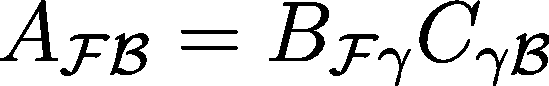
\includegraphics[width=0.5\textwidth]{assets/proxy_2.pdf}
            \end{figure}
        \end{column}

        \begin{column}{0.5\textwidth}
            \begin{figure}
                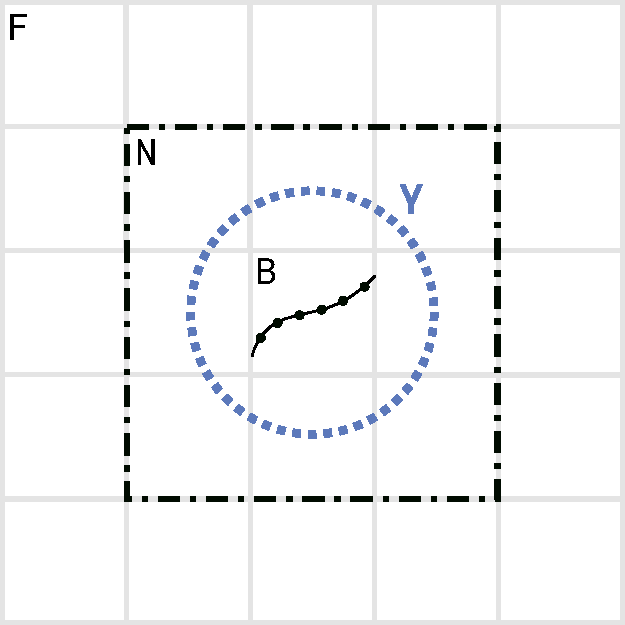
\includegraphics[width=\textwidth]{assets/proxy.pdf}
            \end{figure}
        \end{column}
    \end{columns}

\end{frame}

\begin{frame}
    \frametitle{Proxy Compression II}

    \begin{flalign}
        \label{eq:decomposition}
        A_{\mathcal{F}B} = \begin{bmatrix}
            A_{\mathcal{Q}B}\\ A_{\mathcal{P}B}
            \end{bmatrix} = \begin{bmatrix}
            I & 0\\ 0 & B_{\mathcal{P}\gamma}
            \end{bmatrix} \begin{bmatrix}
            A_{\mathcal{Q}B}\\ C_{\gamma B}
            \end{bmatrix}
    \end{flalign}

    % Let's try and formulate the (outgoing) proxy trick for an integral operator.

\end{frame}


\begin{frame}
    \frametitle{Proxy Compression III}
    \begin{flalign}
        \begin{bmatrix}
            A_{\mathcal{Q}B}\\ C_{\gamma B}
            \end{bmatrix} = \begin{bmatrix}
                A_{\mathcal{Q}S}\\ C_{\gamma S}
            \end{bmatrix} \begin{bmatrix}T_{SR}  & 1 \end{bmatrix}
    \end{flalign}

    Where $S$ and $R$ are the skeleton and redundant points respectively. Plugging back into our expression (\ref{eq:decomposition}),

    \begin{flalign}
        \label{eq:compressed}
        A_{\mathcal{F}B} &=
            \begin{bmatrix}
                I & 0\\ 0 & B_{\mathcal{P}\gamma}
            \end{bmatrix}
            \begin{bmatrix}
                 A_{\mathcal{Q}S}\\ C_{\gamma S}
            \end{bmatrix}
            \begin{bmatrix}T_{SR}  & 1 \end{bmatrix} \\
            &=\begin{bmatrix}
                A_{\mathcal{Q}S}\\ B_{\mathcal{P} \gamma}C_{\gamma S}
           \end{bmatrix} \begin{bmatrix}T_{SR}  & 1 \end{bmatrix} \\
           &=  A_{\mathcal{F}S} \begin{bmatrix}T_{SR}  & 1 \end{bmatrix}
    \end{flalign}

\end{frame}


\begin{frame}

    \frametitle{Helmholtz - Sound Hard I}

    \begin{columns}
        \begin{column}{0.5\textwidth}

            Let's consider the exterior acoustic scattering problem in 3D, with sound-hard
            boundary conditions, for low-frequencies.

            \hspace*{0.5pt}

            \centering
            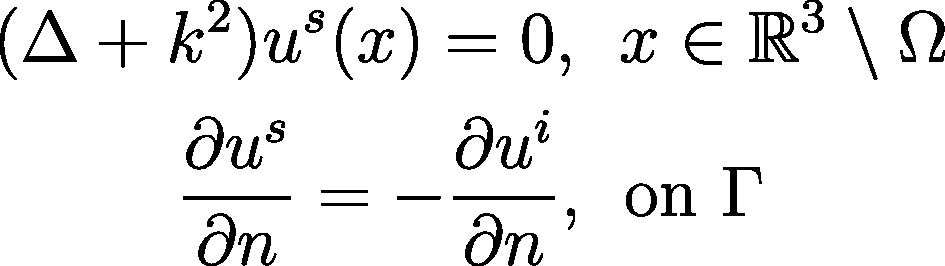
\includegraphics[width=\textwidth]{assets/sound_hard_1.pdf}

        \end{column}

        \begin{column}{0.5\textwidth}
            \begin{center}
                \begin{figure}
                    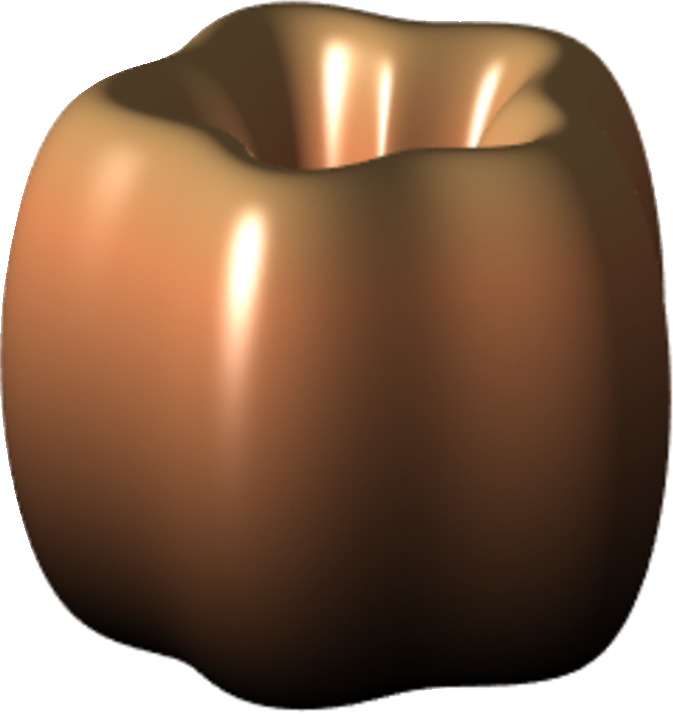
\includegraphics[width=0.6\textwidth]{assets/wiggly_torus.pdf}
                    \caption*{`Wiggly Torus', test geometry}
                \end{figure}
            \end{center}
        \end{column}
\end{columns}

\end{frame}

\begin{frame}
    \frametitle{Helmholtz - Sound Hard II}

    Using a regularised representation, form a boundary integral equation.

    \hspace*{0.5pt}

    \centering
    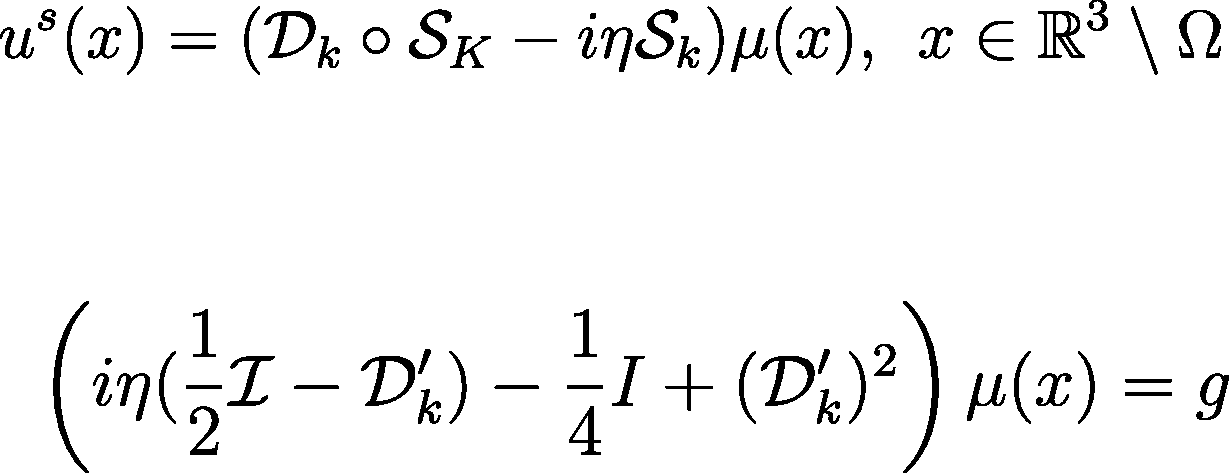
\includegraphics[width=0.6\textwidth]{assets/sound_hard_2.pdf}

\end{frame}

\begin{frame}
    \frametitle{Helmholtz - Sound Hard III}

    Using a Calderon Identity, can form a system of equations, which we proceed
    to discretise.

    \hspace*{0.5pt}

    \centering

    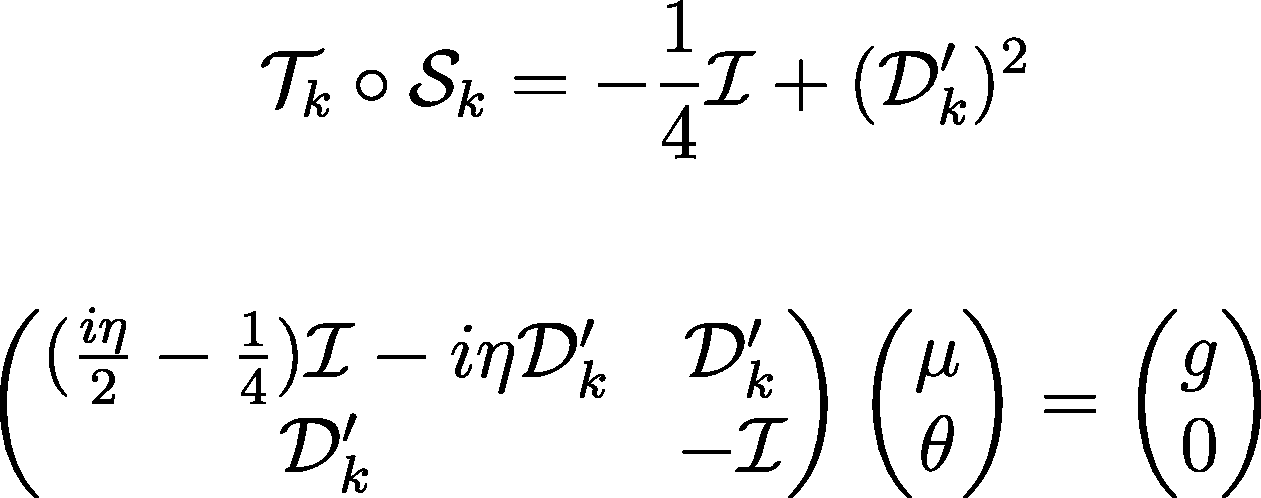
\includegraphics[width=0.6\textwidth]{assets/sound_hard_3.pdf}
\end{frame}

\begin{frame}
    \frametitle{Formulating Proxy Trick I}

    A double-layer potential, due to some unknown density $\psi$, supported on $\tau$,

    \begin{flalign}
        v(x) = \int_{\Gamma \cap B} \frac{\partial \Phi(x, y)}{\partial n(y)} \psi(y) ds(y) := \mathcal{D}\psi, \> \> x \in \mathbb{R}^m \setminus \tau
    \end{flalign}

    solves the Helmholtz equation everywhere it's valid.

    It's normal derivative wrt targets, does not.

    \begin{flalign}
        \frac{\partial v}{\partial n(x)} = \frac{\partial}{\partial n(x)} \int_{\Gamma \cap B} \frac{\partial \Phi(x, y)}{\partial n(y)} \psi(y)ds(y) := \mathcal{T}\psi, \> \> x \in \Gamma \cap \mathcal{F}
    \end{flalign}

\end{frame}

\begin{frame}
    \frametitle{Formulating Proxy Trick II}
    However, we can separate out the normal part of the derivative,

    \begin{flalign}
        \frac{\partial v}{\partial n(x)} = n(x) \cdot \nabla_x \int_{\Gamma \cap B} \frac{\partial \Phi(x, y)}{\partial n(y)} \psi(y)ds(y) := n \cdot w
    \end{flalign}

    The function

    \begin{flalign}
        w(x) = \nabla_x \int_{\Gamma \cap B} \frac{\partial \Phi(x, y)}{\partial n(y)} \psi(y)ds(y) := \nabla_x \mathcal{D}\psi
    \end{flalign}

    Does satisfy our PDE, everywhere.
\end{frame}

\begin{frame}
    \frametitle{Formulating Proxy Trick III}
    Consider an associated boundary value problem for just a single component of $\tilde{w}$ that satisfies,

    \begin{flalign}
        &(\Delta + k^2)\tilde{w} = 0, \> \> x \in \mathbb{R}^m \setminus D \\
        &\tilde{w} = w_1(x) \\
        &\text{A radiation condition at } \infty
    \end{flalign}

    A combined field representation might be nice, as we know it has good properties,

    \begin{flalign}
        \tilde{w} = (\mathcal{D} - ik \mathcal{S})_{\mathcal{F}\gamma} \mu
    \end{flalign}
\end{frame}

\begin{frame}
    \frametitle{Formulating Proxy Trick IV}

    Forming the boundary integral equation, and plugging back into the representation for $\tilde{w}$,

    \begin{flalign}
        \tilde{w} &=  (\mathcal{D} - ik \mathcal{S})_{\mathcal{F} \gamma}(\frac{1}{2}\mathcal{I} + \mathcal{D} - ik \mathcal{S})_{\gamma \gamma}^{-1}w_1 \\
        &= (\mathcal{D} - ik \mathcal{S})_{\mathcal{F} \gamma}(\frac{1}{2}\mathcal{I} + \mathcal{D} - ik \mathcal{S})_{\gamma \gamma}^{-1} \nabla_1 \mathcal{D}_{\gamma B} \psi_\gamma \\
        &\equiv B_{\mathcal{F}\gamma} C_{\gamma B} \psi_\gamma
    \end{flalign}

    where we identify,

    \begin{flalign}
        C_{\gamma B} = \nabla_1 \mathcal{D}_{\gamma B}
    \end{flalign}
\end{frame}

\begin{frame}
    \frametitle{Formulating Proxy Trick V}
    We end up having to compress
   \begin{flalign}
     [\nabla_1 \mathcal{D}_{\gamma B} , \nabla_2 \mathcal{D}_{\gamma B} , \nabla_3 \mathcal{D}_{\gamma B}]
   \end{flalign}
    for the outgoing problem.
\end{frame}


\begin{frame}

    \frametitle{Helmholtz - Sound Hard, Numerical Results I}

    \begin{columns}
        \begin{column}{0.5\textwidth}
            Experiment where density is generated by 50 random charged placed inside the torus.
        \end{column}
        \begin{column}{0.5\textwidth}
            \begin{figure}
                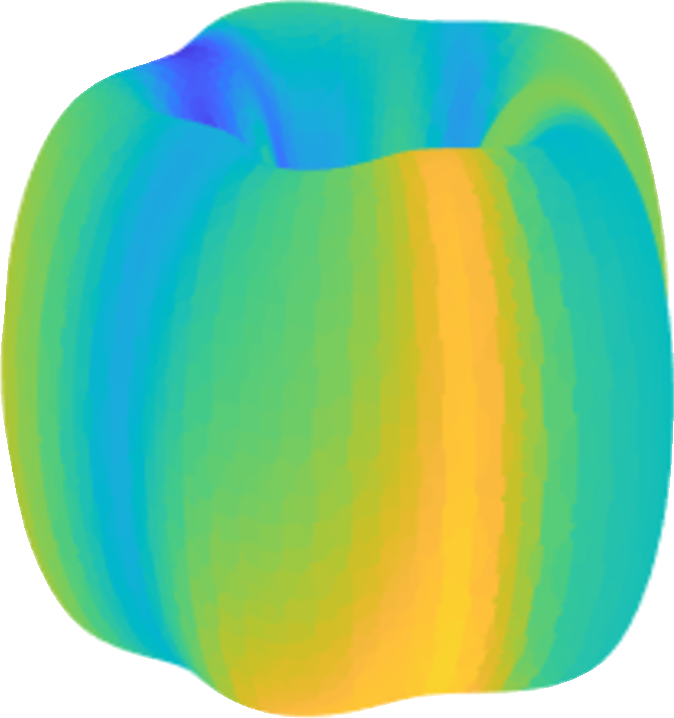
\includegraphics[width=0.6\textwidth]{assets/wiggly_torus_solved.pdf}
            \caption*{Real component of density solved for $p=4$, $N_{\text{patch}} = 200$
                $N = 3000$.
            }
            \end{figure}
        \end{column}
    \end{columns}

\end{frame}

\begin{frame}
    \frametitle{Helmholtz - Sound Hard, Numerical Results II}

    \begin{figure}
        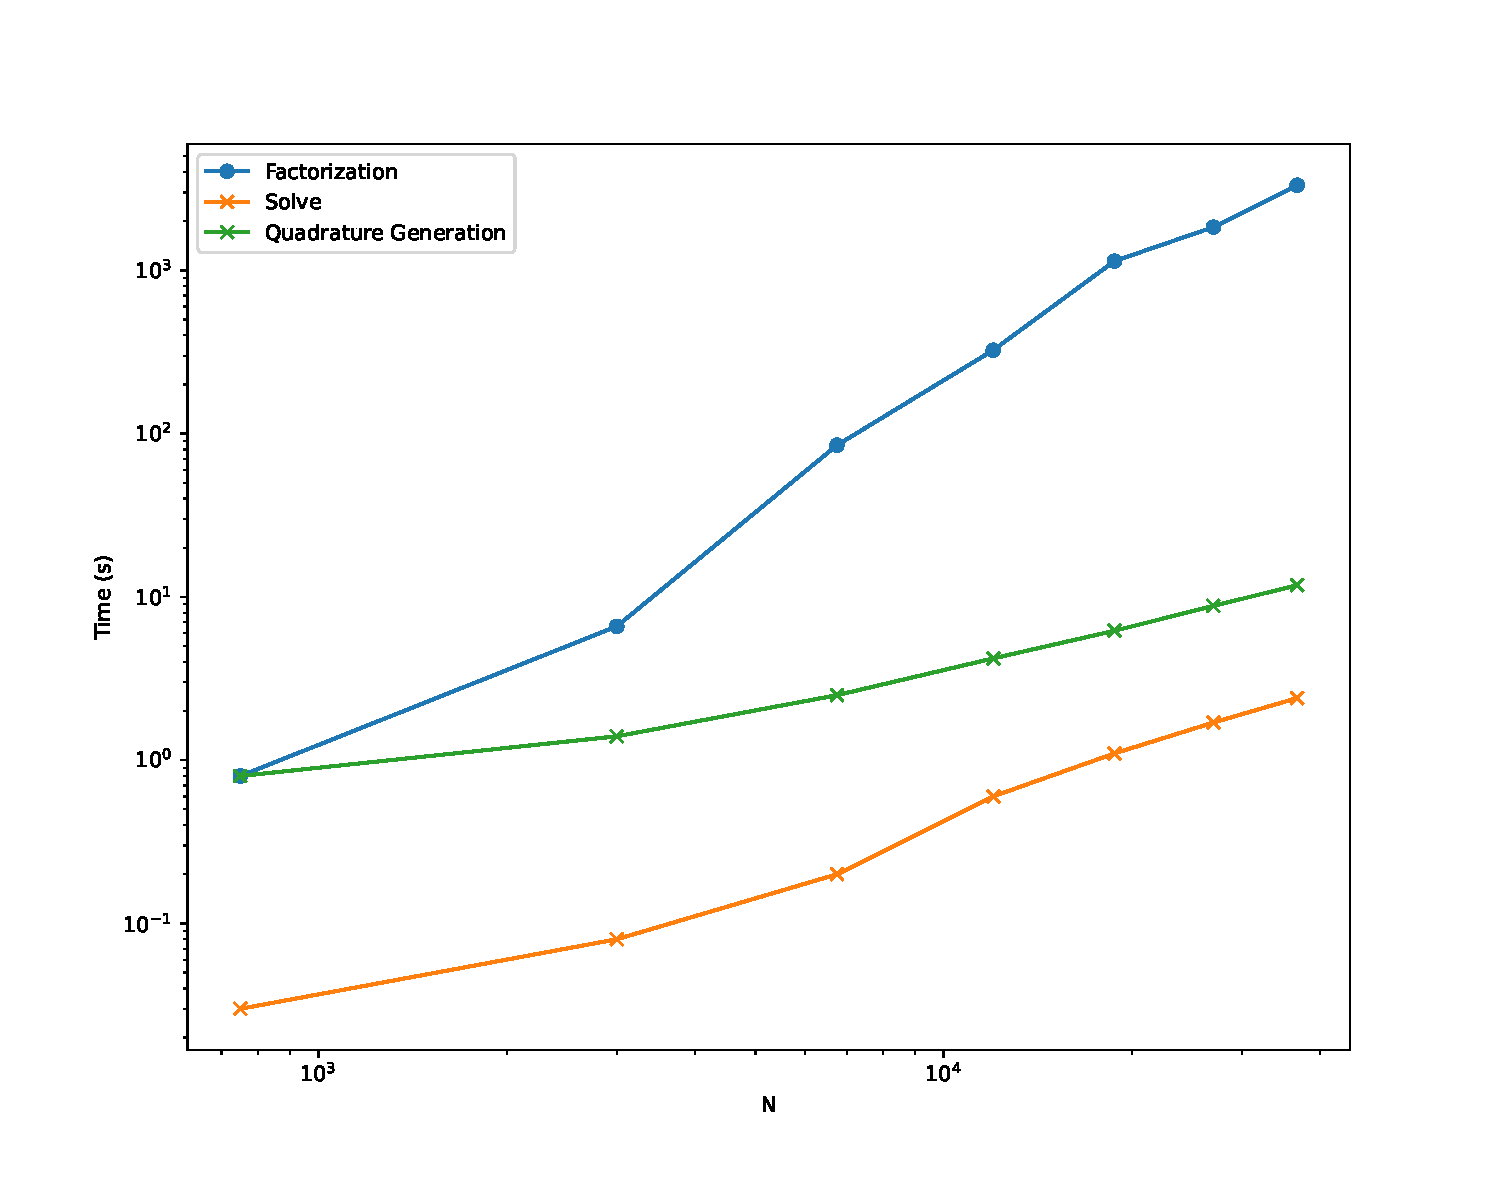
\includegraphics[width=\textwidth]{assets/scaling.pdf}
    \end{figure}
\end{frame}

% \begin{frame}

%     \frametitle{Helmholtz - Transmission}

% \end{frame}


% \begin{frame}

%     \frametitle{Towards Maxwell}

%     \centering
%     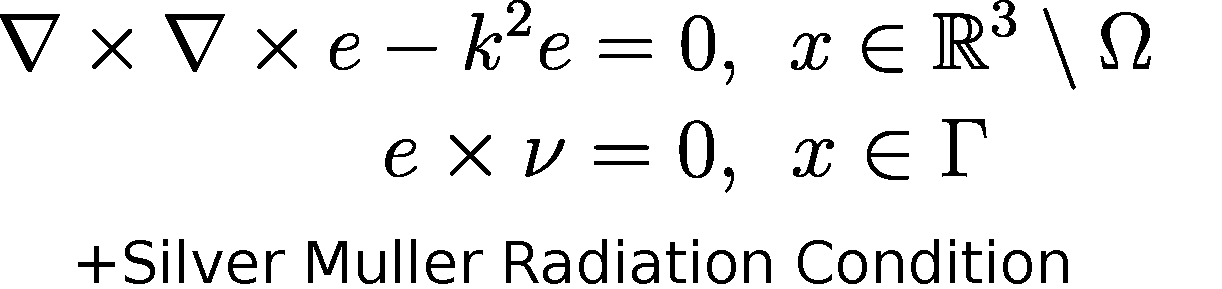
\includegraphics[width=0.6\textwidth]{assets/maxwell_scattering.pdf}

% \end{frame}